

In this exercise two-subsystems are considered in the form
\begin{align}
    \dot{x} =& A_1 x + B_1 u_1 \label{eq:ex2_subsystemx} \\
    \dot{z} =& A_2 z + B_2 u_2. \label{eq:ex2_subsystemz}
\end{align}
Here, $x$ and $z$ the states of the first and second subsystem respectively and with
\begin{align*}
    A_1 = \begin{bmatrix}56 & -20 \\ 0 & 100 \end{bmatrix},& \; \; B_1 = \begin{bmatrix} 0 \\ 1 \end{bmatrix} \\
    A_2 = \begin{bmatrix}-21 & 10 \\ -2 & 30 \end{bmatrix},& \; \; B_2 = \begin{bmatrix} 0 \\ 1 \end{bmatrix}
\end{align*}

For these two sub-systems, there is one actuator that can only actuate on of the systems at a time. When system \eqref{eq:ex2_subsystemx} is actuated we have $u_1 = K_1 \xi$ and $u_2 = K_2 \xi$ if system \eqref{eq:ex2_subsystemz} is actuated. Here $\xi = \begin{bmatrix} x^T \\ z^T \end{bmatrix}$.

\subsection{Exercise 2a}
Since there is one actuator that can only serve one of both subsystems, these systems can be written into a switched linear system in the form
\begin{equation}
    \begin{matrix}
    \dot{\xi} = M_1 \xi \\
    \dot{\xi} = M_2 \xi
    \end{matrix}
    \label{eq:ex2a_SLS}
\end{equation}
After substitution of $u_1$ and $u_2$ in equation \ref{eq:ex2_subsystemx} and \ref{eq:ex2_subsystemz} respectively this results in
\begin{equation*}
    M_1 = \begin{bmatrix}
    A_1 & O \\ O & A_2 \end{bmatrix} + \begin{bmatrix} B_1 \\ O \end{bmatrix}K_1 \; \; \text{and} \; \: M_2 = \begin{bmatrix}
    A_1 & O \\ O & A_2 \end{bmatrix} + \begin{bmatrix} O \\ B_2 \end{bmatrix}K_1
\end{equation*}

\subsection{Exercise 2b}
The SLS introduced in equation \eqref{eq:ex2a_SLS} under periodic switching of the actuator can be considered as a hybrid automaton. With $\tau_1$ the amount of time units that the actuator is serving the first sub-system \eqref{eq:ex2_subsystemx} and $\tau_2$ the amount of time units the actuator is serving the second sub-system \eqref{eq:ex2_subsystemz}. The period of the switching thus equals to $\tau = \tau_1 + \tau_2$. A modelled hybrid automaton looks as:

\begin{figure}[H]
    \centering
    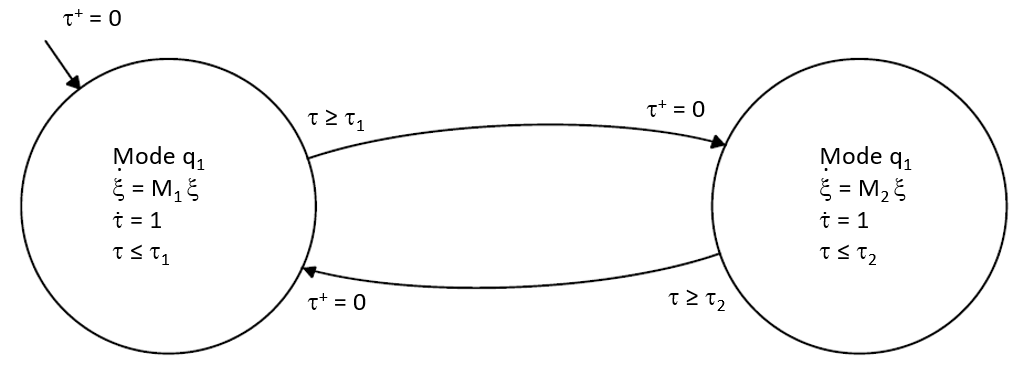
\includegraphics[width=0.8\textwidth]{Images/ex2b_hybridautomaton.PNG}
    \caption{Hybrid automaton of SLS in equation \eqref{eq:ex2a_SLS}}
    \label{fig:ex2b_hybridautomaton}
\end{figure}

\subsection{Exercise 2c}

